\clearpage
\begin{figure*}[t]
    \centering
    \counterwithin{figure}{section}
    \renewcommand\thefigure{C\arabic{figure}}
    \begin{subfigure}[t]{0.95\linewidth}
    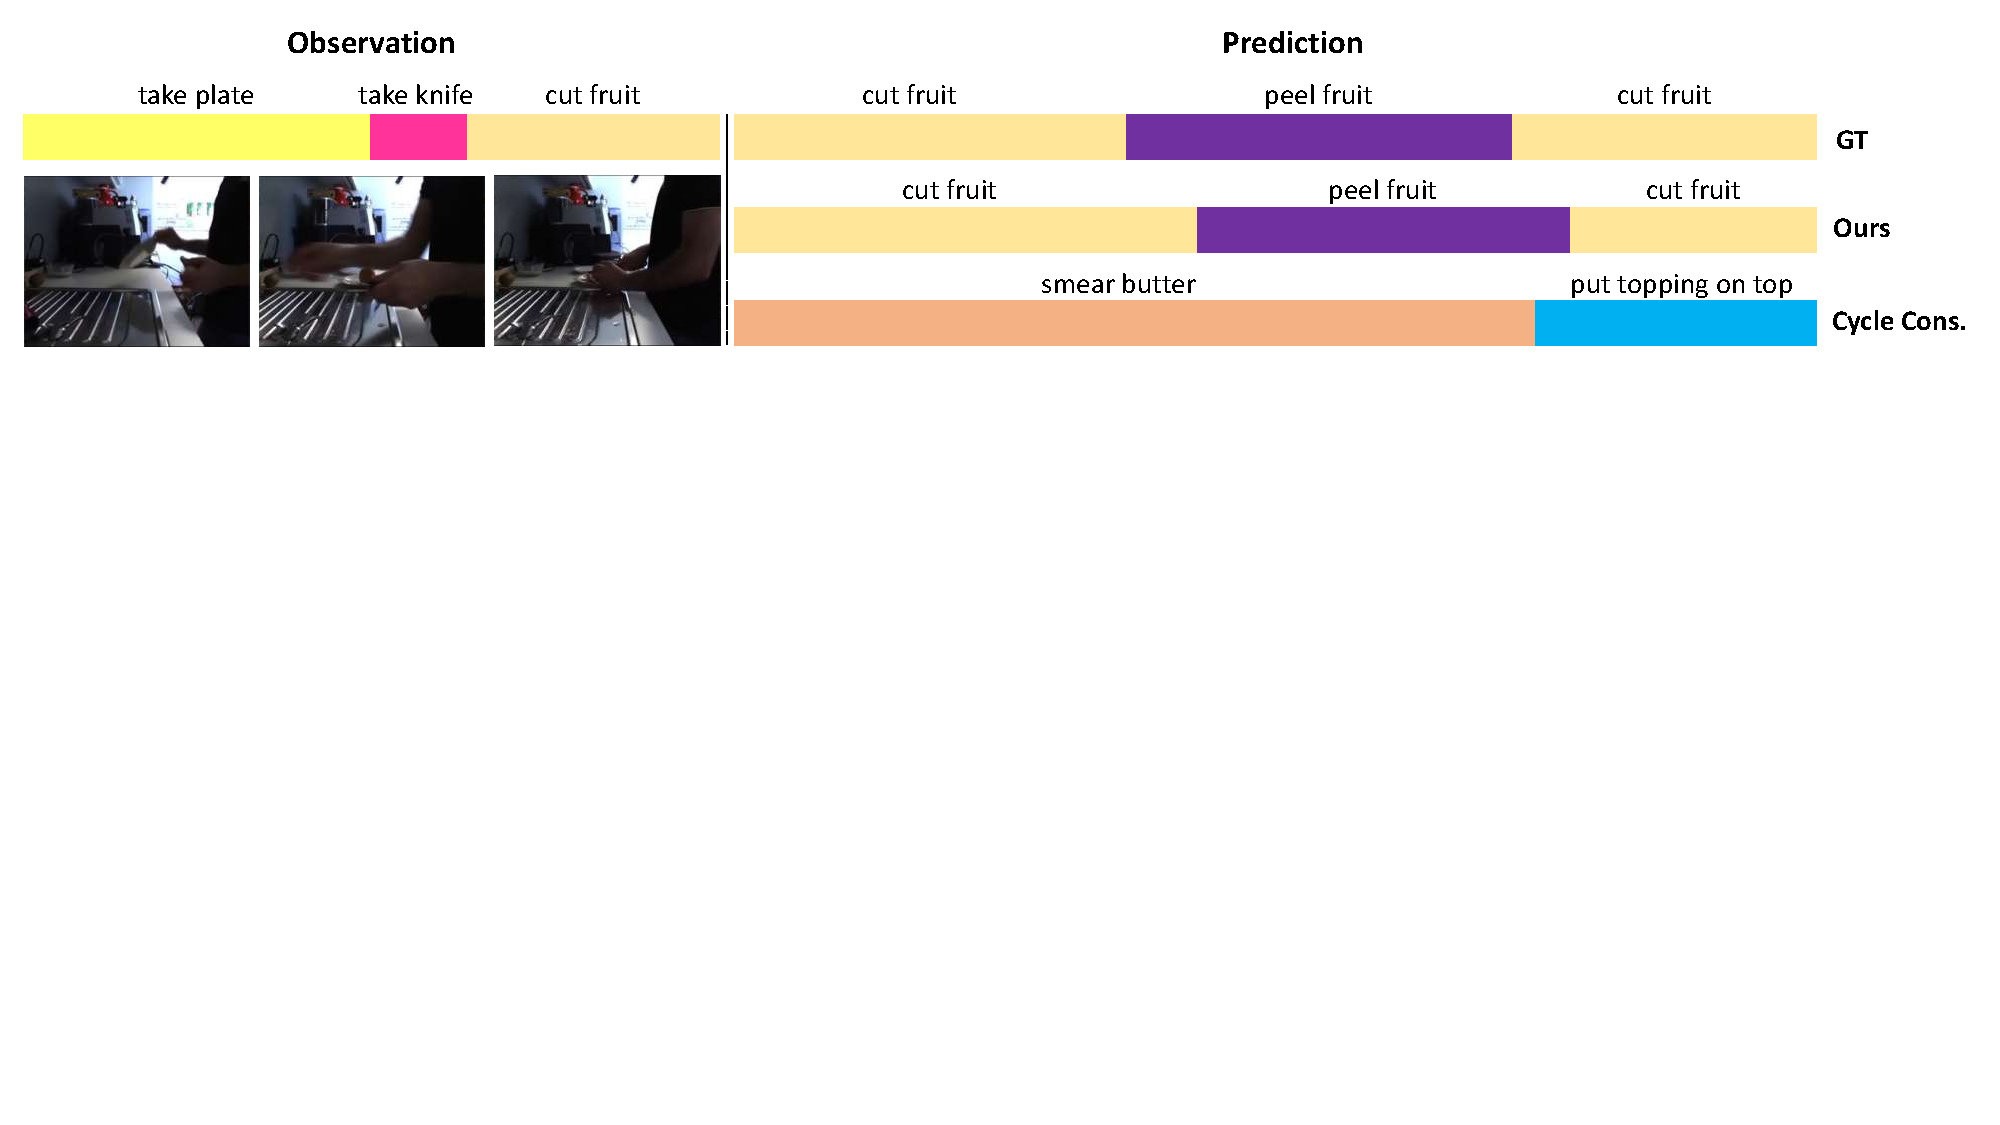
\includegraphics[width=\columnwidth]{Figures/pdf/squal4_compressed.pdf}
    \counterwithin{figure}{section}
    \renewcommand\thefigure{S\arabic{figure}}
    \vspace{-4mm}
    \caption{Activity: salad}
    \label{fig:s5a}
    \end{subfigure}
    
    \begin{subfigure}[t]{0.95\linewidth}
    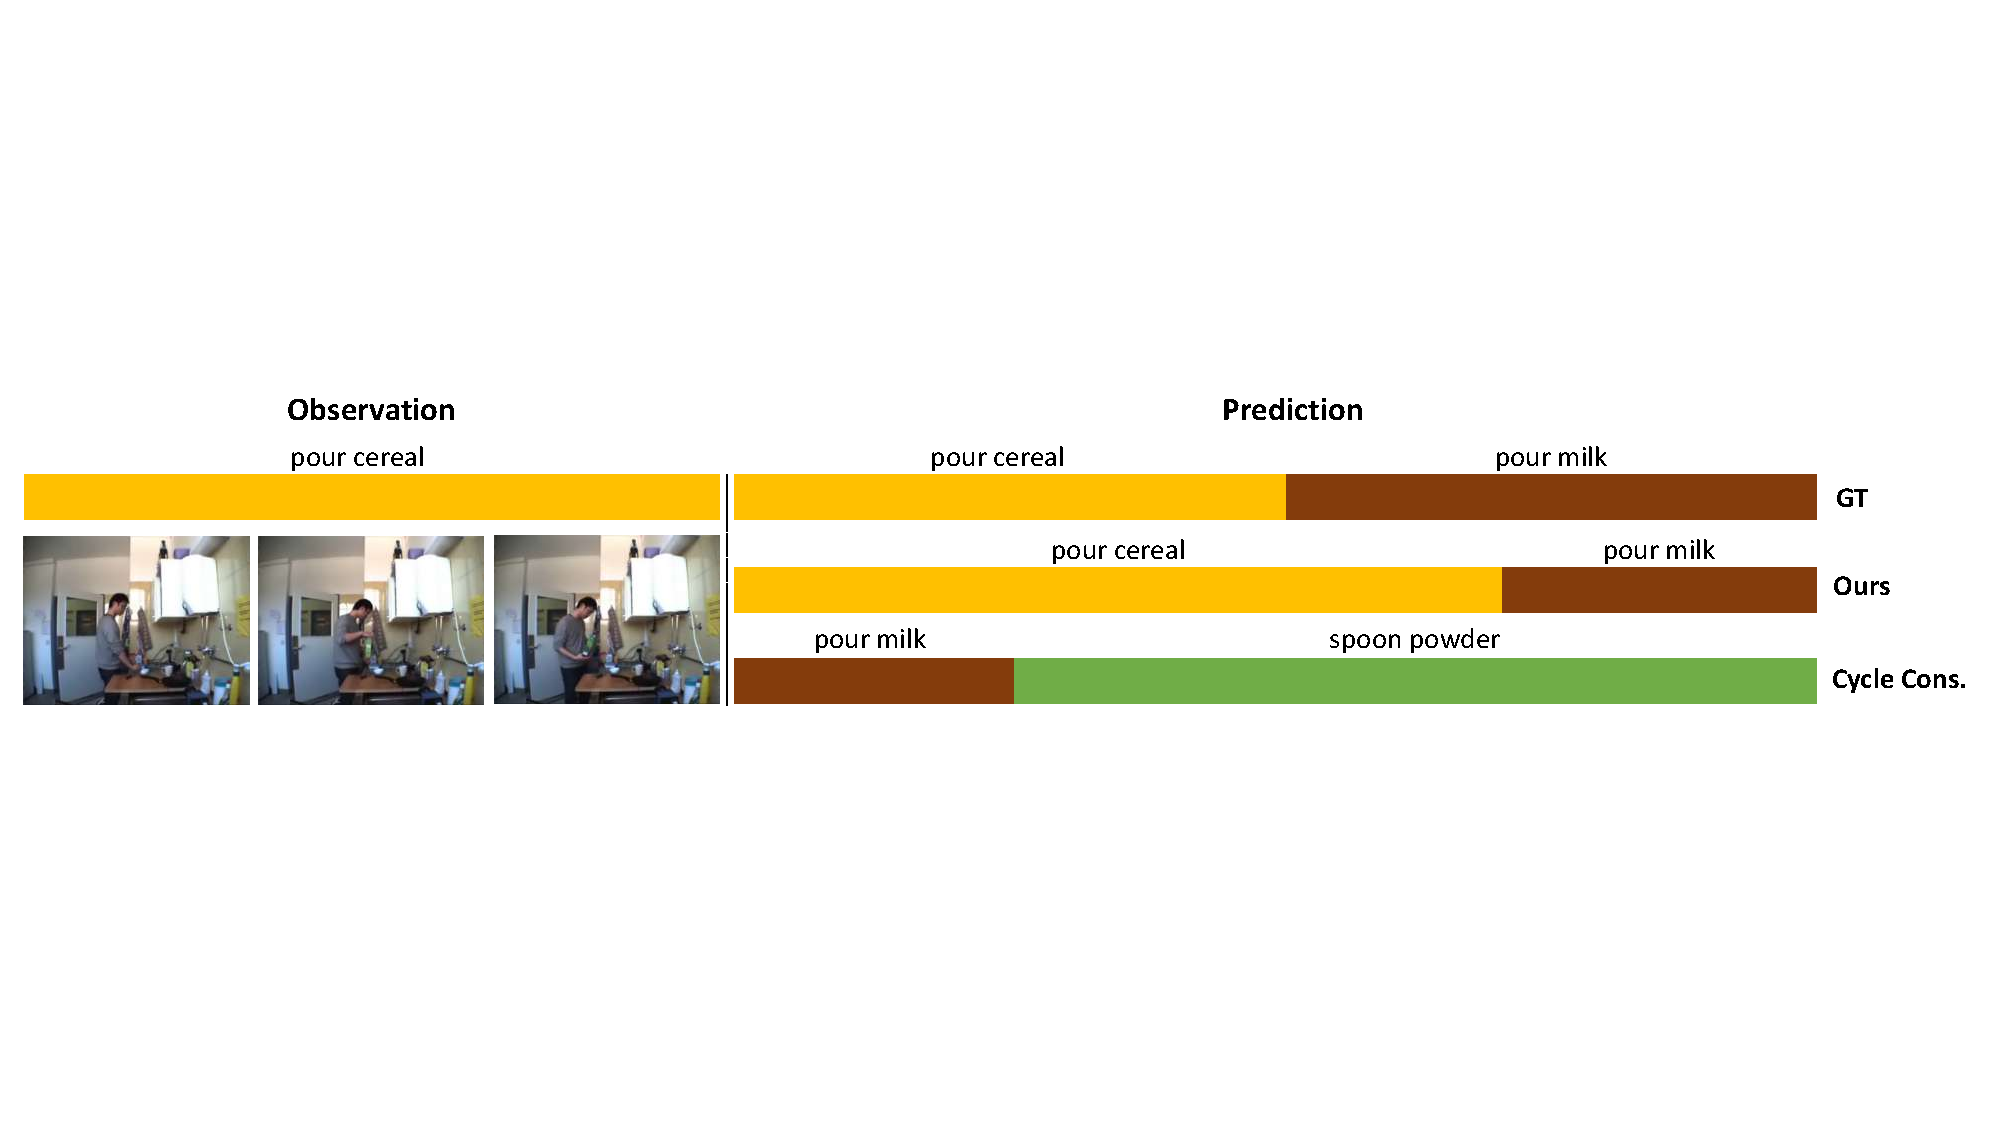
\includegraphics[width=\columnwidth]{Figures/pdf/squal2_compressed.pdf}
    \counterwithin{figure}{section}
    \renewcommand\thefigure{S\arabic{figure}}
    \vspace{-4mm}
    \caption{Activity: cereal}
    \label{fig:s5b}
    \end{subfigure}

    \begin{subfigure}[t]{0.95\linewidth}
    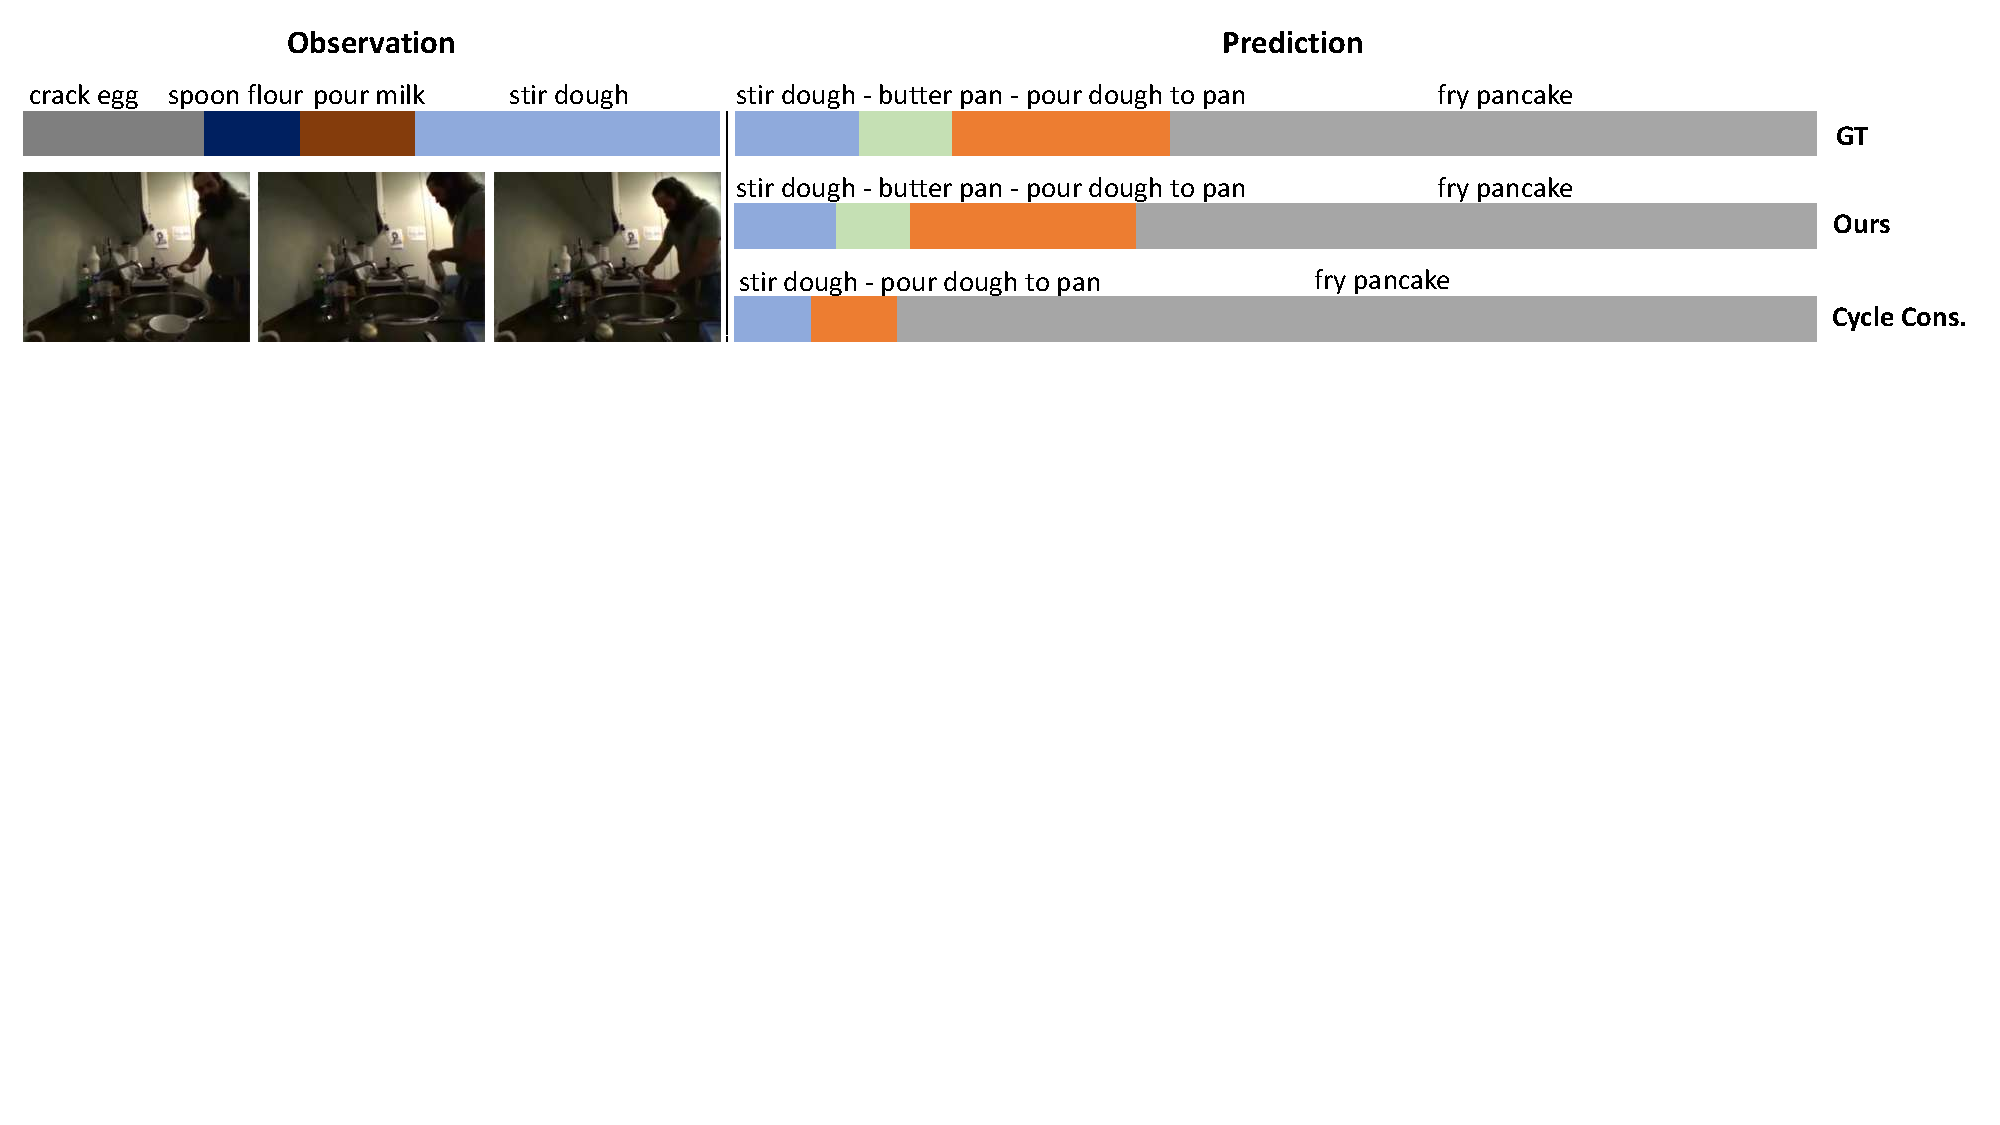
\includegraphics[width=\columnwidth]{Figures/pdf/squal1_compressed.pdf}
    \counterwithin{figure}{section}
    \renewcommand\thefigure{S\arabic{figure}}
    \vspace{-4mm}
    \caption{Activity: pancake}
    \label{fig:s5c}
    \end{subfigure}
    
    \begin{subfigure}[t]{0.95\linewidth}
    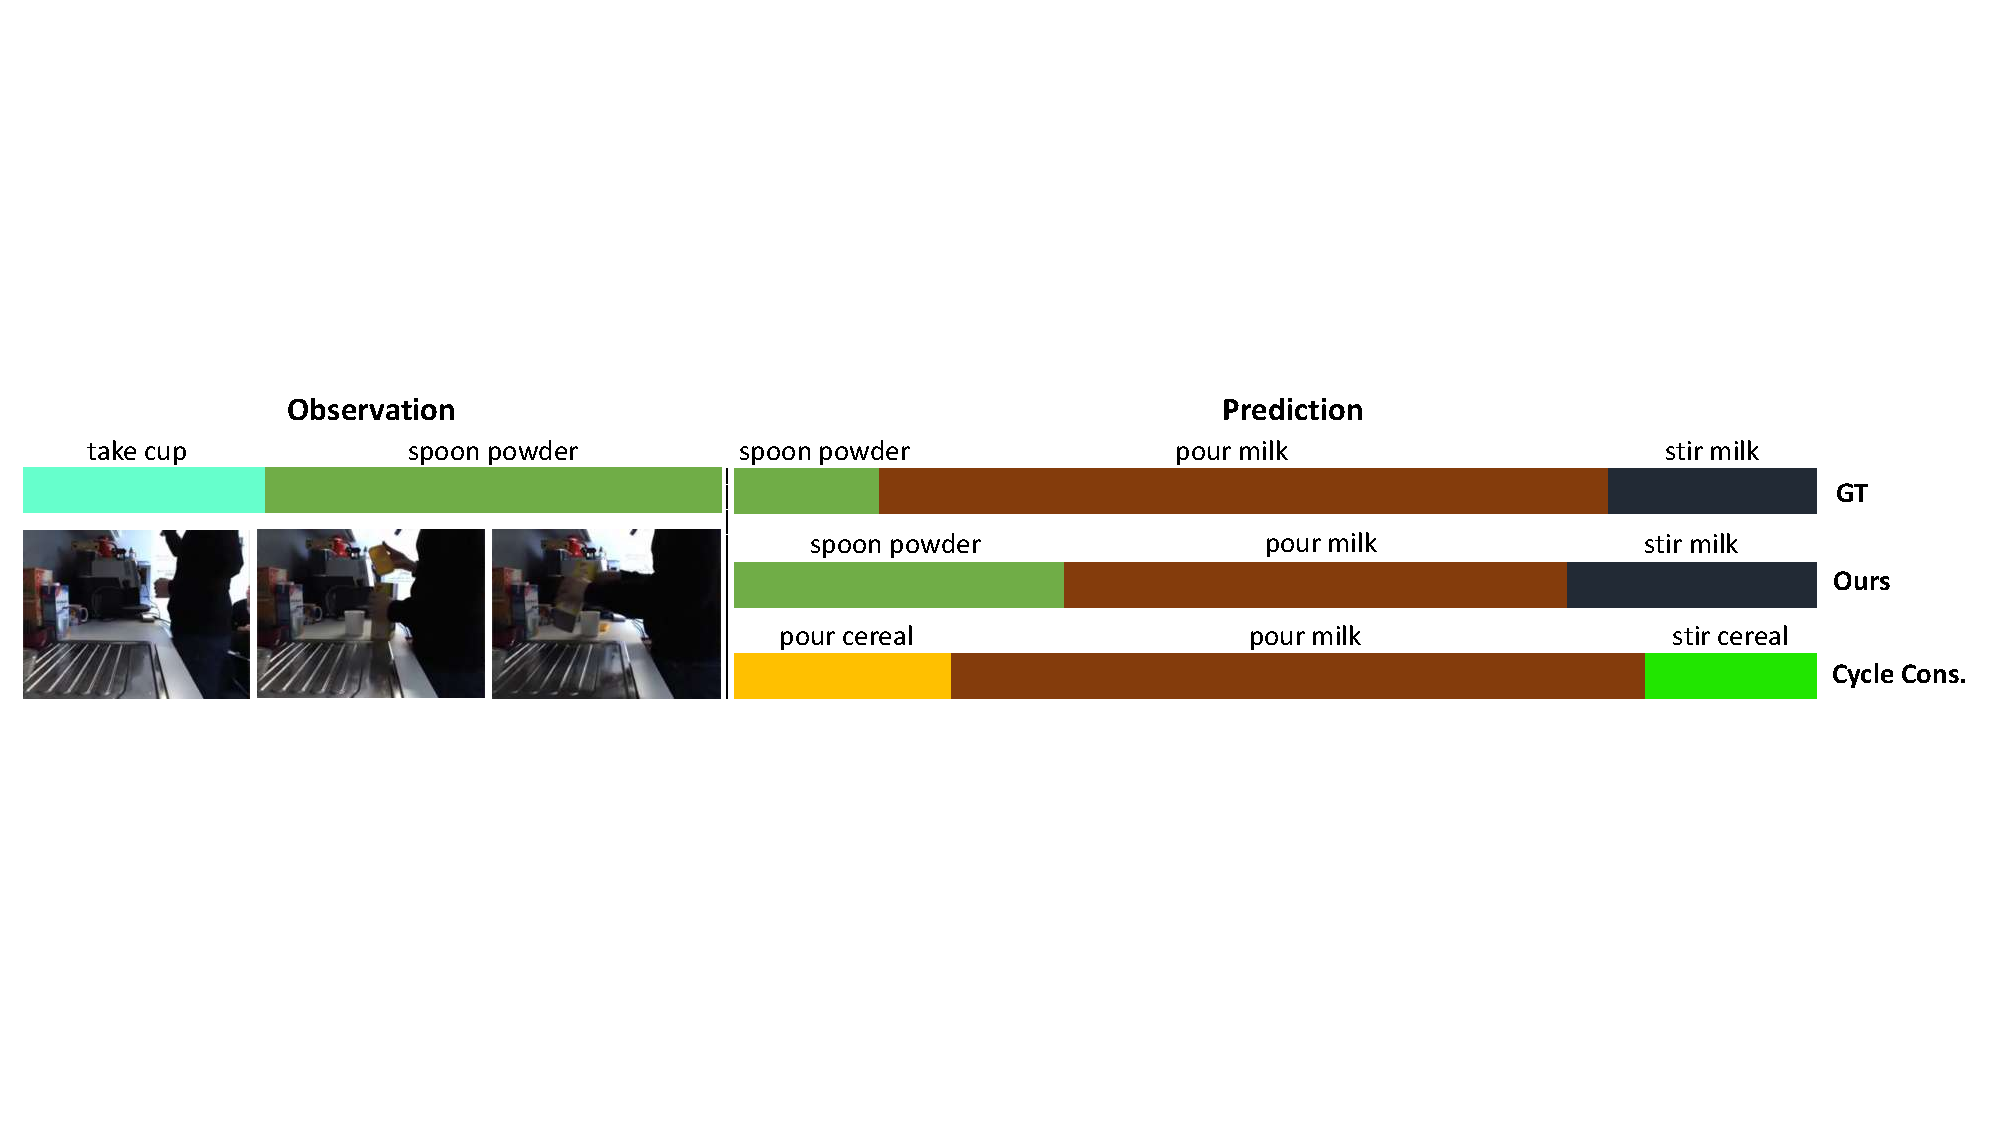
\includegraphics[width=\columnwidth]{Figures/pdf/squal5_compressed.pdf}
    \counterwithin{figure}{section}
    \renewcommand\thefigure{S\arabic{figure}}
    \vspace{-4mm}
    \caption{Activity: milk}
    \label{fig:s5d}
    \end{subfigure}
    
    \begin{subfigure}[t]{0.95\linewidth}
    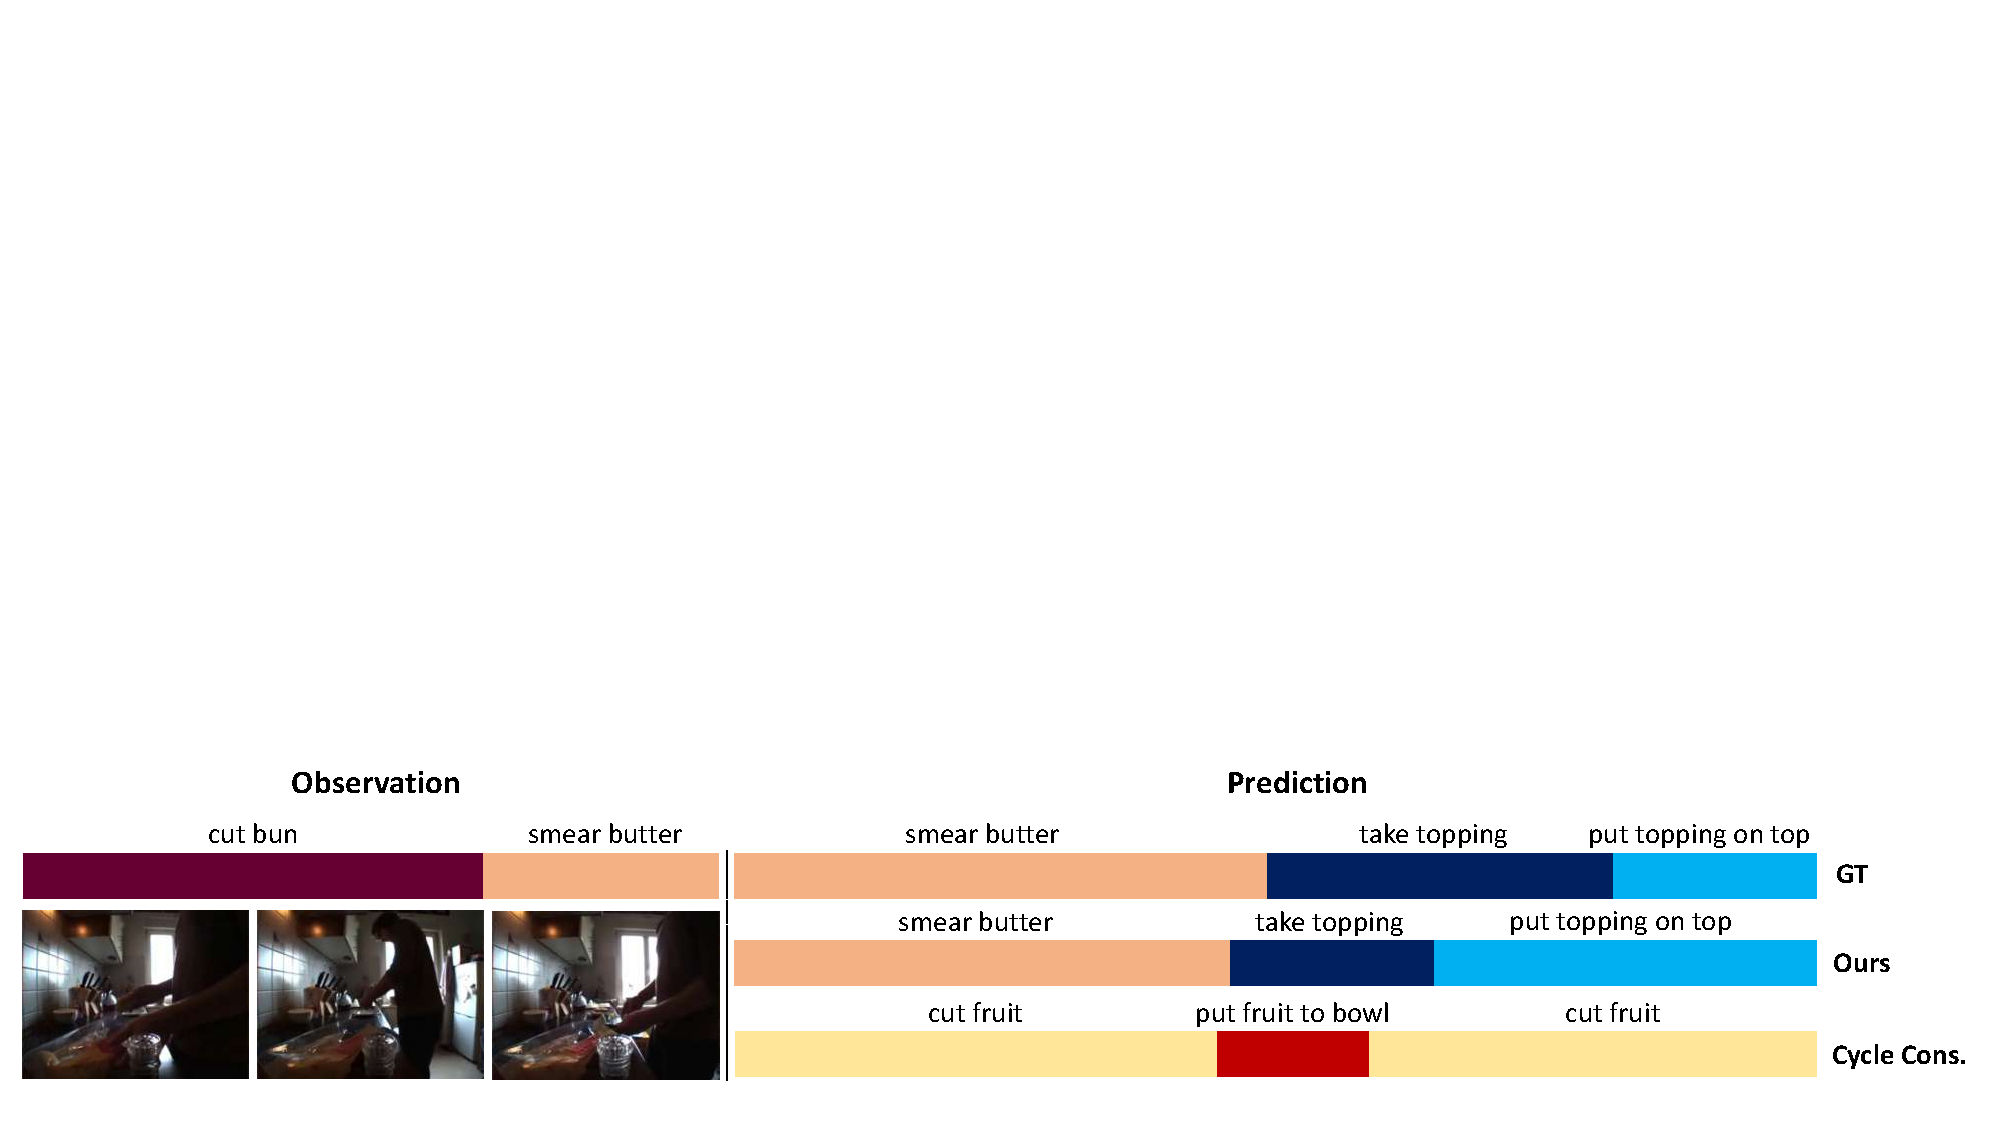
\includegraphics[width=\columnwidth]{Figures/pdf/squal3_compressed.pdf}
    \counterwithin{figure}{section}
    \renewcommand\thefigure{S\arabic{figure}}
    \vspace{-4mm}
    \caption{Activity: pancake}
    \label{fig:s5e}
    \end{subfigure}
\vspace{-2mm}
\counterwithin{figure}{section}
\renewcommand\thefigure{S\arabic{figure}}
\caption{\textbf{Qualitative results on Breakfast}. Each subfigure visualizes the ground truth label and the prediction results of the \ours and cycle consistency model proposed from Farha~\etal~\cite{farha2020long}. We set $ \alpha $ as 0.3 and $ \beta $ as 0.5 in this experiment. We decode action labels and durations to the frame-wise action classes. Each color in the color bar indicates an action label written above. Best viewed in color.}
\vspace{40mm}
 \label{fig:sup_qual}
\end{figure*}